\clearpage
\section{Quantum Models}
\label{sec:quantum_models}

The rationale behind building a quantum version of a Game Theory and/or Statistics problem lays in bringing phenomena like quantum superposition, and entanglement into known frameworks. Converting known classical problems into quantum games is relevant to the familiarize with the potential differences these models bring.

\subsection{Quantum Roulette}
\label{subsec:quantum_roulette}

In the arbitrary $N$-State quantum roulette,\cite{Salimi2009} presented a $N$-State roulette model using permutation matrices. 

This model is interesting because in captures the usage of permutation matrices to manipulate and change the state of the system.

To verify this model with two players we developed a Matlab simulation \ref{ap:c}, that followed the steps taken in \cite{Salimi2009}.

The game in represented in a $N$-Dimensional Hilbert Space. There is a basis in the space that represents each of the equally probable entries as shown in \ref{eq:roulette_1}. In a sense this is a generalization of a quantum coin flip that is also used in Section \ref{sec:quantum_walk_line}.
\begin{equation}
\label{eq:roulette_1}
\vert1\rangle=\left[\begin{array}{c}
1\\
0\\
0\\
\vdots\\
0
\end{array}\right],\:\vert2\rangle=\left[\begin{array}{c}
0\\
1\\
0\\
\vdots\\
0
\end{array}\right],\:\ldots,\:\vert N\rangle=\left[\begin{array}{c}
0\\
0\\
0\\
\vdots\\
1
\end{array}\right]
\end{equation}

Each state transition is obtained using a permutation matrix denoted by $P^{i}$. There are $N!$ permutation matrices, so in the particular case of having a $3$-State roulette, there are $6$ possible transition choices. The classical strategy considered will rely on choosing an arbitrary probability distribution, that verifies\ref{eq:roulette_2}, and that maps the usage of the permutation matrices. This step will not affect the density matrix ($\rho$) of the roulette\ref{eq:roulette_3}.

\begin{equation}
\label{eq:roulette_3}
\rho=\frac{1}{N!}\sum_{i=0}^{N!-1}P^{i}
\end{equation}

\begin{equation}
\label{eq:roulette_2}
\sum_{i=0}^{N!-1}p_{i}=1
\end{equation}

The density matrix is diagonalizable by a Discrete Fourier Transform because it is a kind of circulant matrix\cite{Davis1994}, as we can see in \ref{eq:roulette_4}. In \ref{eq:roulette_4} $\lambda_{k}$ are eigenvalues of $\rho$. $\lambda_{1}=1$
while $\lambda_{2}=\lambda_{3}=\lambda_{k}=\lambda_{N-1}=0$. Each column
$i$ of the Fourier matrix will represent a eigenvector $\vert\lambda_{i}\rangle$.
If we construct the diagonalizing matrix by rotating the columns of
the Fourier Matrix we can obtain the projection states as in \ref{eq:roulette_5}.

\begin{equation}
\label{eq:roulette_4}
F^{\dagger}\rho F=\left[\begin{array}{c}
\lambda_{1}\\
0\\
0\\
\vdots\\
0
\end{array}\begin{array}{c}
0\\
\lambda_{2}\\
0\\
\vdots\\
0
\end{array}\begin{array}{c}
\ldots\\
\ldots\\
\ldots\\
\ddots\\
\ldots
\end{array}\begin{array}{c}
0\\
0\\
0\\
\vdots\\
\lambda_{N-1}
\end{array}\right]
\end{equation}



\begin{equation}
\label{eq:roulette_5}
\vert1\rangle\langle1\vert=\left[\begin{array}{c}
1\\
0\\
0\\
\vdots\\
0
\end{array}\begin{array}{c}
0\\
0\\
0\\
\vdots\\
0
\end{array}\begin{array}{c}
\ldots\\
\ldots\\
\ldots\\
\ddots\\
\ldots
\end{array}\begin{array}{c}
0\\
0\\
0\\
\vdots\\
0
\end{array}\right]=F^{\dagger}\rho F
\end{equation}


The quantum strategy advantage in this case is that the first player
will not alter the density matrix\ref{eq:roulette_6}.

\begin{equation}
\label{eq:roulette_6}
\rho=\sum_{i=0}^{N!-1}p_{i}P^{i}\rho P^{i\dagger},\;\sum_{i=0}^{N!-1}p_{i}=1
\end{equation}

This means that if the second player knows the initial state and the first player plays with a classical strategy, thus never modifying the system density matrix, the second player will be able to manipulate the game under optimal conditions. This result is confirms the demonstration done in \cite{Meyer1999}; on Quantum Strategies, where in a classical $2$ player zero-sum game, if one player adopts a quantum strategy, she increases her chances of winning the game.

\clearpage
\subsection{Prisoner's Dilemma}
\label{sebsec:related_work_prisioners_dillama}

The Prisoner's Dilemma is a classic example of a game that can be represented
in normal form\cite{Osborne2004}. This problem has received a great deal of attention
because, in its simple form, rational individuals will seem to deviate
from solutions that would represent the best social interest,
the Pareto Optinal solution. In this game the Pareto Optimal solution
is not a Nash Equilibrium. The Prisoner's Dilemma can be formulated
as it follows:

\begin{quotation}

Two suspects of being partners in a crime are arrested. The police
needs more evidence in order to prosecute the prisoners. So each
prisoner is locked in solitary confinement and has no means of communicating
with the other suspect. The police will then try to extort a confession
from the prisoners. A bargain will be proposed to the suspects:
\begin{itemize}
\item If the suspect testifies against the other suspect (Defects) and the other denies, he will
go free and the second will get three years sentence.
\item If they both testify against one another (both Defect), both will
be convicted and they will get two years.
\item In case both suspects deny the involvement (both Cooperate) of the
other, they will get a one year sentence.
\end{itemize}
\end{quotation}

A matrix representation of the problem is in Table \ref{tab:prisionersdillema_tab1}, here the payoff represented by the letter $R$ would be the standard reward for the game, $T$ would be the temptation to deviate from a cooperation profile, $P$ represents the punishment when both entities do not cooperate, and finally $S$ would be a sucker's payoff. A particular case for this problem is represented in Table \ref{tab:prisionersdillema_tab2}. In each cell of the matrix we have a pair of the expected utility for the players for every outcome. A higher utility represents a more desirable state.

In this game the Pareto Optimal solution happens when both players chose to Cooperate (the pair (2,2) in Table \ref{tab:prisionersdillema_tab2}). However both players have the incentive to Defect, because regardless what the opponent chooses they will have always a strictly higher payoff. Defecting becomes a dominant strategy in the Prisioner's Dillema and the outcome $(Defect, Defect)$ is a Nash Equilibrium to the game. 

\begin{center}
\begin{table}[h]
\begin{centering}
\begin{tabular}{ccc}
\hline 
 & Player 2: C & Player 2: D\tabularnewline
\hline 
Player 1: C & (R,R) & (S,T)\tabularnewline
Player 1: D & (T,S) & (P,P)\tabularnewline
\hline 
\end{tabular}
\par\end{centering}

\caption{The canonical normal form representation for the Prisoner's Dilemma must respect $T>R>P>S$.}
\label{tab:prisionersdillema_tab1}
\end{table}
\par\end{center}

\begin{center}
\begin{table}[h]
\begin{centering}
\begin{tabular}{ccc}
\hline 
 & Player 2: C & Player 2: D\tabularnewline
\hline 
Player 1: C & (2,2) & (0,3)\tabularnewline
Player 1: D & (3,0) & (1,1)\tabularnewline
\hline 
\end{tabular}
\par\end{centering}

\caption{One possible normal form representation of Prisoner's Dilemma.}
\label{tab:prisionersdillema_tab2}
\end{table}
\par\end{center}


\subsubsection{Quantum Prisoner's Dilemma}
\label{subsubsec:quantum_prisioners_dillema}

The importance of the Prisoner's Dilemma for the study of Game Theory made it a prime target for investigation in Quantum Game Theory. The problem has been modelled several times \cite{Eisert2008}\cite{Letters2002}. Therefore we will use it in order to exemplify and consolidate the definition described in Section \ref{sec:background_quantum_game_theory}\cite{Fra2011a}. 

Each player $i$ in the quantum version of Prisoner's Dilemma will be able to manipulate one qubit ($\varphi_{1}$ and $\varphi_{2}$) in Equations \ref{eq:quantum_prisioner_m1} and \ref{eq:quantum_prisioner_m2}, with the unitary operators (shown in Equation \ref{eq:operators_prisioneiros_quanticos}). The  classical strategies: Cooperate (C), and Defect (D). $C$ is represented in the sub-set $\mathcal{U}_{j}$ (Equation \ref{eq:operators_prisioneiros_quanticosmiaurons}) . $D$, also known as the Bit-flip operator ($\sigma_{x}$), is not represented in the restricted space proposed in \cite{Eisert2008}\cite{Fra2011a}. $D^{y}$ is an alternative to $D$ in the sub-set $\mathcal{U}$.

\begin{equation}
\varphi_{1}=a_{0}\vert0\rangle+a_{1}\vert1\rangle,\sum_{i=0}^{1}\vert a_{i}\vert^{2}=1
\label{eq:quantum_prisioner_m1}
\end{equation}


\begin{equation}
\varphi_{2}=b_{0}\vert0\rangle+b_{1}\vert1\rangle,\sum_{j=0}^{1}\vert b_{j}\vert^{2}=1
\label{eq:quantum_prisioner_m2}
\end{equation}

\begin{equation}
\mathcal{U}_{j} ( \theta,\phi) = \left[\begin{array}{cc}
cos(\frac{\phi}{2}) & e^{i\phi}sin(\frac{\phi}{2})\\
-e^{-i\phi}sin(\frac{\phi}{2}) & cos(\frac{\phi}{2})
\end{array}\right] , j \in \{ 1, 2\}, \theta \in ( 0, \pi ) , \phi \in ( 0, \frac{\pi}{2})
\label{eq:operators_prisioneiros_quanticos}
\end{equation}

\begin{equation}
\begin{cases}C= 
U_{j}(0, 0)=\left[\begin{array}{cc}
1 & 0\\
0 & 1
\end{array}\right]\\
D=\left[\begin{array}{cc}
0 & 1\\
1 & 0
\end{array}\right] \\
D^{y}= U_{j}(\pi, 0)=\left[\begin{array}{cc}
0 & 1\\
-1 & 0
\end{array}\right]
\end{cases} , j \in \{ 1, 2 \}
\label{eq:operators_prisioneiros_quanticosmiaurons}
\end{equation}

The system that holds the game is represented in a $\mathcal{H}^{4}$. Each basis ($\vert 1\rangle, \vert 2\rangle, \vert 3\rangle, \vert 4\rangle$), represents a final outcome as Table \ref{tab:prisioners_m} suggests.

\begin{table}
\begin{centering}
\begin{tabular}{ccc}
\hline 
$\bigotimes$ & C-$\vert 0\rangle$ & D-$\vert 1\rangle$\tabularnewline
\hline 
C-$\vert 0\rangle$ & $\vert 0,0\rangle$ & $\vert 0,1\rangle$\tabularnewline
D-$\vert 1\rangle$ & $\vert 1,0\rangle$ & $\vert 1,1\rangle$\tabularnewline
\hline 
\end{tabular}
\par\end{centering}

\caption{Construction of the basis for the game space; $\mathcal{H}^{4}$.}
\label{tab:prisioners_m}
\end{table}



The fundamental difference from the classical version lies in the way the initial state is formulated in Equation and que strategies the players might use\ref{eq:estado_inicial_prisioneiro}. We will entangle our state by applying the gate $\mathcal{J}$ \cite{Letters2002}\cite{Eisert2008}. 

The parameter $\gamma$ becomes a way to measure the entanglement in the system\cite{Eisert2008}.

\begin{equation}
\label{eq:matrix_exponencial_esoterica}
\mathcal{J}=exp\left\{ i\frac{\gamma}{2}\left[\begin{array}{cc}
0 & 1\\
1 & 0
\end{array}\right]\otimes\left[\begin{array}{cc}
0 & 1\\
1 & 0
\end{array}\right]\right\}
\end{equation} 

\begin{equation}
\label{eq:estado_inicial_prisioneiro}
%\vert \psi_{in}(\gamma) \rangle= cos( \frac{\gamma}{2})\vert 00\rangle+ isin(\frac{\gamma}{2})\vert 11 \rangle, \gamma \in (0,\pi)
\begin{split}
\vert\psi_{in}(\gamma)\rangle=exp\left\{ i\frac{\gamma}{2}\left[\begin{array}{cc}
0 & 1\\
1 & 0
\end{array}\right]\otimes\left[\begin{array}{cc}
0 & 1\\
1 & 0
\end{array}\right]\right\} \vert00\rangle \\
=cos(\frac{\gamma}{2})\vert00\rangle+isin(\frac{\gamma}{2})\vert11\rangle,\gamma\in(0,\pi)
\end{split}
\end{equation}

\begin{equation}
\vert\psi_{fin}\rangle= \mathcal{J}^{\dagger} \otimes_{i=1}^{2}\mathcal{U}_{i}\vert\psi_{in}\rangle
\label{eq:finalstate_prisioneersdilemma}
\end{equation}

The entanglement in quantum game theory can be viewed as an intrinsic unbreakable contract. Furthermore measuring an entangled state will cause the wave function that describes the state to collapse. Before measuring the final result we will de-entangle the system by applying the operator $\mathcal{J}^{\dagger}$, as shown in Equation \ref{eq:finalstate_prisioneersdilemma}.

The utility functions for each player is calculated by projecting the final state in each base and attributing a real number to each measurement, as in equation.
In order to compare a classical version with this quantum model, the real numbers assigned are those in the classical example in Table \ref{tab:prisionersdillema_tab1}, and the basis are presented in Table \ref{tab:prisioners_m}.

\begin{equation}
E_{0}(\vert\psi_{fin}\rangle)=2\times\vert\langle00\vert\psi_{fin}\rangle\vert^{2}+3\times\vert\langle10\vert\psi_{fin}\rangle\vert^{2}+1\times\vert\langle11\vert\psi_{fin}\rangle\vert^{2}
\end{equation}


\begin{equation}
E_{1}(\vert\psi_{fin}\rangle)=2\times\vert\langle00\vert\psi_{fin}\rangle\vert^{2}+3\times\vert\langle01\vert\psi_{fin}\rangle\vert^{2}+1\times\vert\langle11\vert\psi_{fin}\rangle\vert^{2}
\end{equation}



The gate $\mathcal{J}$ is chosen to be commutative with the super-operators created by the tensor product of the classical strategies C and D: $ [ \mathcal{J} , C \otimes C ] = 0 $, $ [ \mathcal{J} , C \otimes D ] = 0 $, $ [ \mathcal{J} , D \otimes C ] = 0 $, and $ [ \mathcal{J} , D \otimes D ] = 0 $. 

This condition implies that any pair of strategies in the sub-set $S_{0} = \{ \mathcal{U} ( \theta , 0) , \theta \in (0, \pi) \}$ is the equivalent of a classical mixed strategy when $\gamma = 0$; the joint probability associated with measuring a outcome $(\delta_{1}, \delta_{2}) \in \{ (C, C), (C, D), (D, C), (D, D) \} $ ( $ P( \delta_{1} , \delta_{2} ) = { \vert \langle \delta_{1} , \delta_{2} \vert \psi_{fin} \rangle \vert }^{2} $ ), becomes $ P( \delta_{1} , \delta_{2} ) =P( \delta_{1} ) P( \delta_{2})$, with $P(C) = cos^{2}(\frac{ \theta }{2})$, and $P(D) = 1 - P(C)$\cite{Eisert2008}.

If the parameter $\phi$ in the operator $U_{j}(\theta ,\phi)$ and the entanglement coefitient differ from $0$ we are able to explore quantum strategies that have no counterpart in the classical domain.

\cite{Eisert2008} finds that the pair of strategies $( \mathcal{U}( 0 , \frac{\pi}{2}), \mathcal{U}( 0 , \frac{\pi}{2}))$ for $\gamma = \frac{\pi}{2}$ yield  a payoff of $(2,2)$, which is a Nash equilibrium and it is Pareto Optimal when we have a restricted space described by $\mathcal{U}$\ref{eq:operators_prisioneiros_quanticos}. If we allow the operator $D$\ref{eq:operators_prisioneiros_quanticosmiaurons} however, according to \cite{Letters2002} there is no quantum pure strategy Nash Equilibrium, when the entanglement is maximal, $\mathcal{U}(\pi, 0)$ is the optimal counter-strategy for $C$ (represented by the identity matrix), $\mathcal{U}(0, \frac{\pi}{2})$ is the optimal counter strategy for $\mathcal{U}(\pi, 0)$, $D$ becomes the optimal counter-strategy for $\mathcal{U}(0, \frac{\pi}{2})$, and $C$ becomes an optimal counter strategy for $D$\cite{Du}.




\begin{comment}

\begin{table}[ht!]
\begin{center}
\begin{tabular}{cc}
  \num\putindeepbox[7pt]{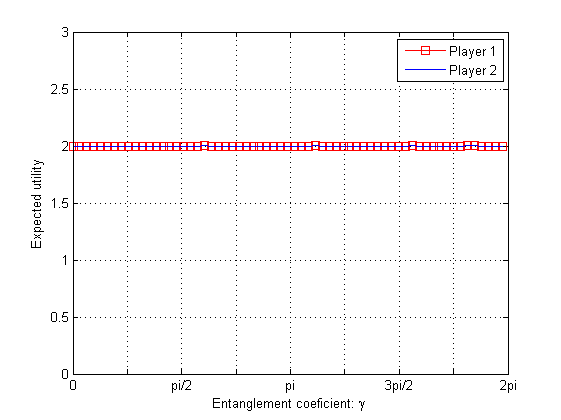
\includegraphics[scale=0.46]{prisionersdillema/II.PNG}}
    & \num\putindeepbox[7pt]{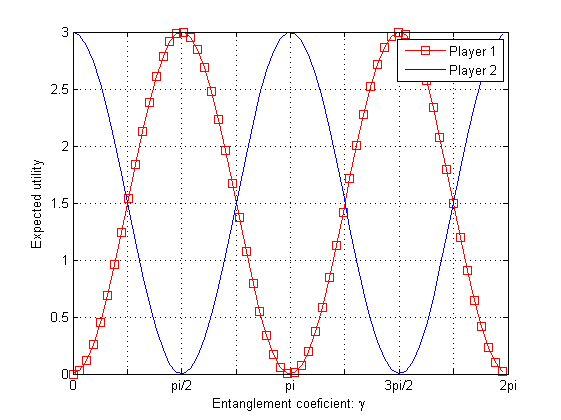
\includegraphics[scale=0.46]{prisionersdillema/InotI.PNG}} \\
  \num\putindeepbox[7pt]{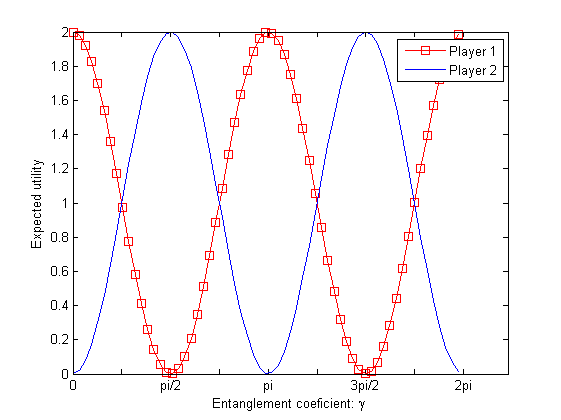
\includegraphics[scale=0.46]{prisionersdillema/notII.PNG}}
    & \num\putindeepbox[7pt]{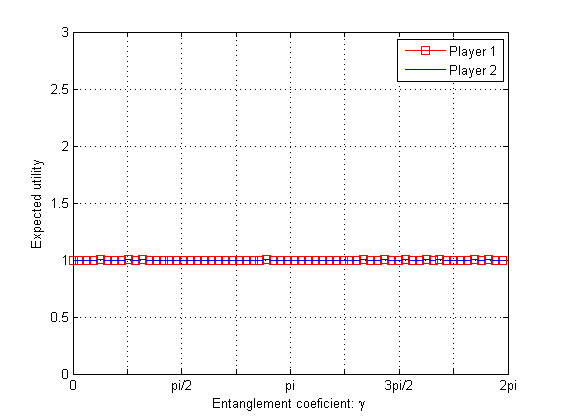
\includegraphics[scale=0.46]{prisionersdillema/notInotI.PNG}} \\
\end{tabular}
\caption{Expected utility for players 1 and 2 giving the entanglement coefficient $\gamma$ used in preparing the initial state. a) Player 1: Cooperates, Player 2: Cooperates;
b) Player 1: Cooperates, Player 2: Defects; c) Player 1: Defects, Player 2: Cooperates; d) Player 1: Defects, Player 2: Defects. }
\label{tab:prisiones_m_4}
\end{center}
 \end{table}

\end{comment}

%\clearpage
\subsection{Ultimatum Game}
\label{subsec:ultimatumquantum}





The ultimatum game is an example of an extensive form game where two players interact in order to divide a sum of money.

A finite amount of money (or other finite resource), is given to the players, and player $1$ must propose how the money will be divided between the two players. If the second player agrees with the proposal, the resource will be split accordingly. When the player $2$ rejects the proposal, neither player will receive the money.

If we consider that we have 100 coins, the number of coins received can be considered the expected utility associated with the proposal. The first player can either present a fair division (F), where the coins are split evenly, or an unfair division (U) game tree that represents the Ultimatum Game is shown in Figure \ref{fig:ultimatum:gametree}.

\begin{figure}[h]
\centering 
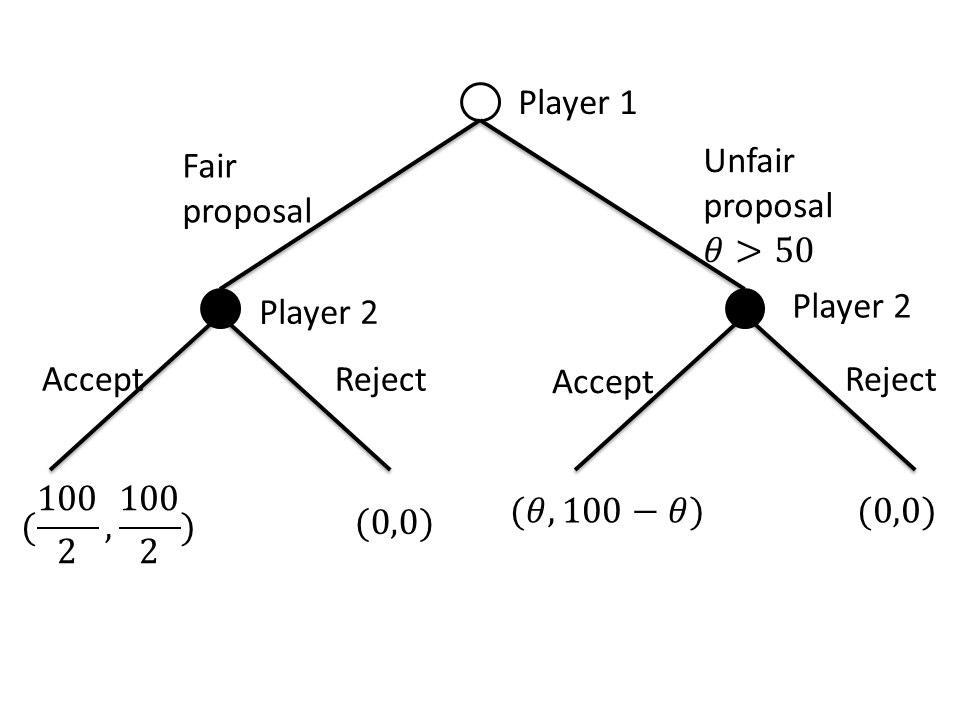
\includegraphics[scale=0.35]{Figures/ultimatum/gametree.png}
\caption{Ultimatum Game representation in the extensive form. }
\label{fig:ultimatum:gametree}
\end{figure}

\subsubsection{Quantum Model}
\label{subsec:ultimatum}

In a ``Quantum information approach to the ultimatum game''\cite{Fra2011} we are presented with a quantization scheme for the ultimatum game that uses the definition of quantum game in Section \ref{sec:background_quantum_game_theory}. 
 They compare that approach to other quantum game definitions, and proposes and compares also quantum  extensive form of the game. 


If we present the game in Figure \ref{fig:ultimatum:gametree} in the normal form we get the matrix represented in Table \ref{tab:tabelaultimatumestoufofida}. The player $2$ has $4$ possible strategies. The strategy $A_{F}R_{U}$ means that the player $2$ will accept a fair division proposed by player $1$ but will reject a unfair division.

 The quantum game representation for this game is $
\Gamma_{Ultimatum}=(\mathcal{H}^{2^{3}},\: 2,\:\vert\psi_{in}\rangle,\:\xi,\:\{\mathcal{U}_{j}\},\:\{E_{i}\})
$. The game system will consist in $3$ qubit, which correspond to the number of actions in the game. Player $1$ will be able to manipulate the qubit $1$, the player $2$ can manipulate the remaining qubits. 


\begin{center}
\begin{table}[h]
\begin{centering}
\begin{tabular}{ccccc}
\hline 
 & Player 2: $A_{F}A_{U}$ & Player 2: $A_{F}R_{U}$ & Player 2: $R_{F}A_{U}$ & Player 2: $R_{F}R_{U}$\tabularnewline
\hline 
Player 1: $F$ & $(50,50)$ & $(50,50)$& $(0,0)$ & $(0,0)$\tabularnewline
Player 1: $U$ & $(\theta,100-\theta)$ & $(0,0)$& $(\theta,100-\theta)$ & $(0,0)$\tabularnewline
\hline 
\end{tabular}
\par\end{centering}

\caption{Normal form representation of the ultimatum game.}
\label{tab:tabelaultimatumestoufofida}
\end{table}
\par\end{center}

The extensive form approach in \cite{Fra2011} allows the differentiation between simultaneous moves and sequential moves. This is accomplished by measuring the game state in order to separate game stages. This "Sequential procedure" uses the L\"{u}ders Rule, a quantum analogous of conditional probability.


The main points discussed in  \cite{Fra2011} Quantum Ultimatum approach are that the game definition presented in Section \ref{sec:background_quantum_game_theory}  makes the game more convenient to analyse than the extensive form approach.






\clearpage
\section{Overview}
\label{sec:related_work_overview}


There are more examples of games that have attracted interest in the Quantum domain. In this overview we are going to present a general picture of the work already done in this field.
 
For example various Models have been proposed to describe a quantum version of the Monty Hall problem\cite{Gill}\cite{Flitney2008}.
This popular problem\cite{Savant1990} is known for its counter-intuitiveness. The problem can be posed as a contest where the player must choose a door (from a set of $3$), and has $\frac{1}{3}$ of probability of getting a prize. After the player has chosen the door, one of the remaining $2$ doors which does not have a prize is opened. The contestant is asked whether is to her advantage to switch her initial choice.

As the host reveals information, the initial set-up is modified. This is an interesting property. Despite being a counter-intuitive problem, a quantum approach to this problem allows an in-depth comparison between the classical measurement and the quantum measurement. The classic Monty Hall problem is modelled using conditional probability and Baye's Rule to learn that it is to the advantage of the contestant to switch doors. In the quantum version, measuring the outcome of the final state yields the result, instead of taking into account the intermediate actions \cite{Fra2011}. In \cite{Gill2002} we can observe the attempt to stick as closely to the classical formulation as possible, the host has a system that is correlated to the game system.

The principal information taken from this problems is that there is not a unique way to model a classical problem\cite{Gill2002}. Therefore, when modelling a classical problem, we need to select properties that could potentially benefit from a quantum approach.

From the point of view of Quantum Cognition (a domain that seeks to introduce Quantum Mechanics Concepts in the field of Cognitive Sciences), these games are approached from the perspective of trying to model the mental state of the players in a quantum manner. The Prisoner's Dilemma is an example of a problem that has been modelled in order to explain discrepancies from the theoretical results of the classical Game Theory approach and the way humans play the game\cite{Pothos2009}. 

One last example worth mention is the quantum approach of the Stackelberg Duopoly problem\cite{Khan2011}\cite{Iqbal2008}. This is an Economics Game Theory model that seeks to represent the interactions of two companies, a market leader and a follower which play sequentially; the leader makes a decision and the follower responds. 


